\subsection{Ciclo de Vida - Metodología - SCRUM}

Scrum es una metodología ágil. Contiene un marco de trabajo adaptable, iterativo, rápido, flexible y eficaz, diseñado para ofrecer un valor considerable de forma rápida a lo largo del proyecto. Para cada proyecto que se aplique esta metodología se debe utilizar los principios scrum que son sus lineamientos básicos para la aplicación de su marco de trabajo y sus aspectos. A continuación, se mencionan las características de los principios y los aspectos del mismo.

\textbf{Principios de Scrum}
\begin{enumerate}
    \item Control del proceso empírico (Empirical Process Control)
    \item Autoorganización (Self-organization)
    \item Colaboración (Collaboration)
    \item Priorización basada en valor (Value-based Prioritization)
    \item Time-boxing
    \item Desarrollo iterativo (Iterative Development)
\end{enumerate}

\textbf{Aspectos de Scrum}
\begin{enumerate}
    \item \textbf{Organización}: Entiende los roles y responsabilidades definidos del proyecto con fines de asegurar la implementación exitosa de Scrum. Los roles de Scrum se dividen en 2 categorías: roles centrales (\textbf{Product Owner}, \textbf{Scrum Master}, \textbf{Equipo Scrum}) y roles no centrales (Interesados del negocio, clientes, usuarios y patrocinadores/sponsors).  
    \item \textbf{Justificación del negocio}: Se lleva a cabo una evaluación adecuada del negocio antes de iniciar el proyecto.  
    \item \textbf{Calidad}: Es la capacidad con la que cuenta el producto o los entregables para cumplir los con los criterios de aceptación y de alcanzar el valor de negocio esperado por el cliente.  
    \item \textbf{Cambio}: Los miembros del equipo del proyecto deben entender que los procesos de desarrollo están diseñados para el cambio.  
    \item \textbf{Riesgo}: Son una serie de eventos inciertos que pueden afectar los objetivos de un proyecto y pueden contribuir a su éxito o fracaso. Los riesgos que puedan tener impacto positivo en el proyecto, son considerados como oportunidades, mientras los riesgos que puedan tener impacto negativo en el proyecto se les conoce como amenazas.
\end{enumerate}

\subsubsection{Fase - Inicio}

\textbf{Visión del proyecto.}

Para administradores, vecinos y propietarios del edificio que necesiten resolver la desorganización y demoras en las gestiones diarias, nuestro \textbf{Sistema de Administración de consorcio} es una plataforma digital centralizada que automatiza liquidación de expensas, facilita la gestión de vecinos, implementa seguridad tanto dentro del edificio como fuera del mismo y agiliza la comunicación entre Inquilinos/propietarios del edificio. A diferencia de métodos manuales como Whatsapp o papel, en \textbf{nuestro sistema se garantiza una transparencia, comunicación rápida and efectiva con un control eficiente} de los recursos del edificio. Hemos identificado a \textbf{Fernández Gabriel Elías} como \textbf{Product Owner} por la visión del proyecto que proporcionó.

\textbf{Identificación del Scrum Master.}

Bajo los criterios de: \textbf{buen liderazgo}, \textbf{asignación de trabajo para los miembros dependiendo de sus habilidades en programación} y \textbf{actitud ante las adversidades}, identificamos a \textbf{Matías Solis Schneeberger} como nuestro \textbf{Scrum Master}, que nos guiará en este proyecto.

\textbf{Formación Equipo Scrum.}

Nuestro \textbf{Product Owner} con la colaboración del \textbf{Scrum Master}, ha seleccionado a \textbf{Escobar Lucas Joel} y \textbf{Nicolás Kern}, como miembros del equipo Scrum.

\textbf{Desarrollo de épicas y creación del backlog priorizado del Producto.}

Con la declaración de la visión del proyecto hemos podido lograr \textbf{desarrollar las épicas esenciales} para nuestro sistema. A continuación se muestran las épicas desarrolladas junto al \textbf{Backlog priorizando el producto.}

\begin{figure}[H]
    \centering
    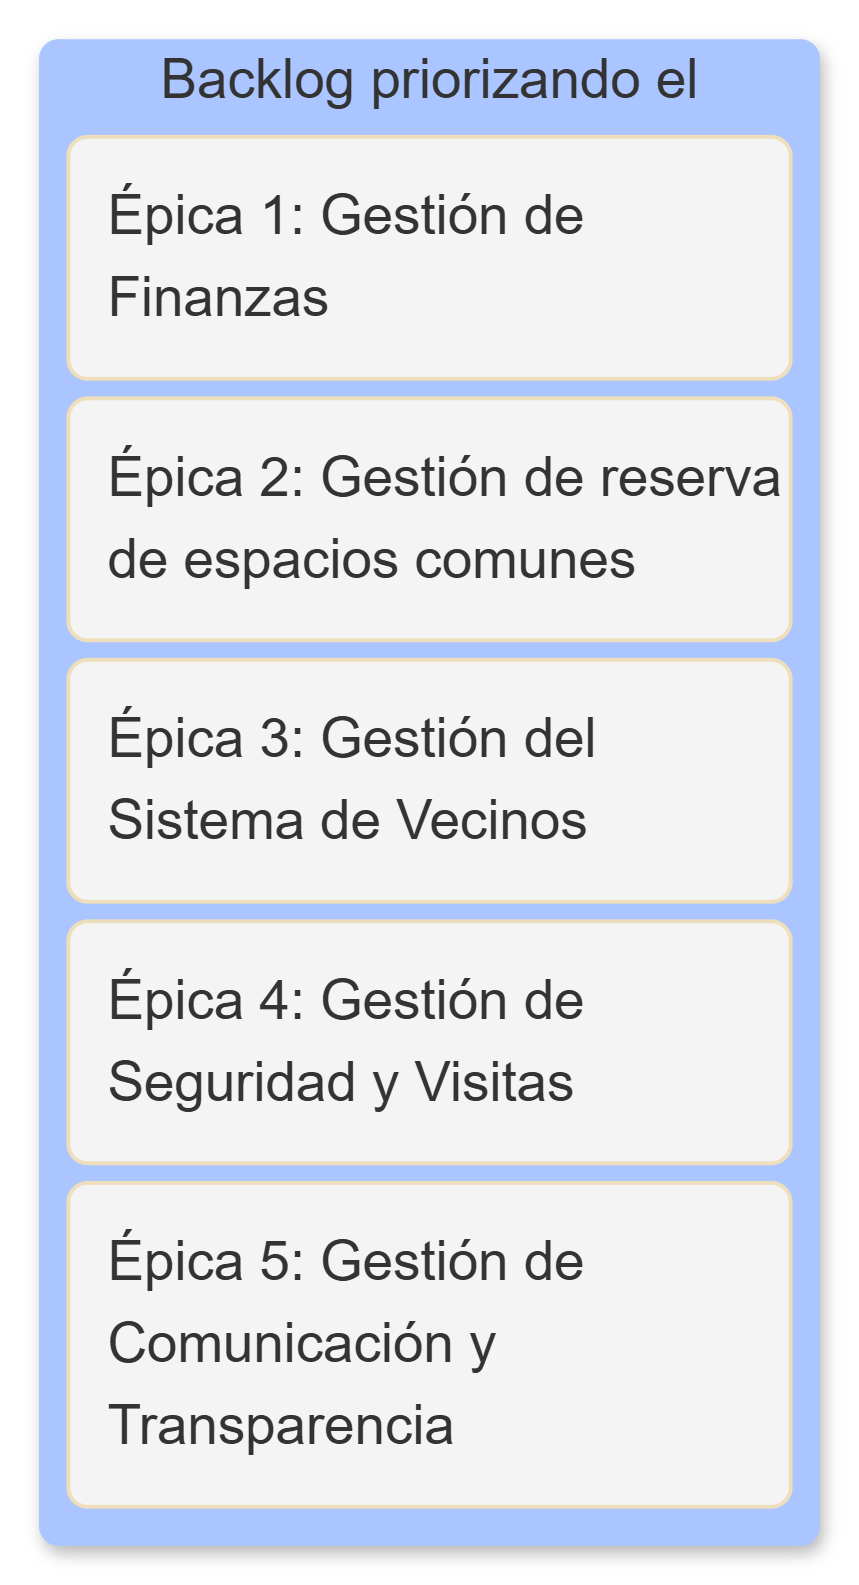
\includegraphics[width=0.313\textwidth]{figures/lista-de-backlog-con-las-epicas.png}
    \caption{Lista de BackLog con las épicas.}
\end{figure}



\textbf{Planificación de la liberación}

Tras el análisis del \textit{Product Backlog}, el Equipo Scrum ha priorizado las entregas basándose en el valor de negocio. Se determinó que el núcleo del sistema es el módulo contable, por lo que la Épica 1 (Gestión de Finanzas) conformará la primera liberación. Las entregas subsecuentes abordarán la gestión de reservas, usuarios, seguridad y comunicación.  

\textbf{Liberación 1: Gestión Financiera Base (Duración: 2 Sprints de 2 semanas)}
Para esta primera entrega, aplicamos una estricta priorización, seleccionando únicamente las Historias de Usuario (HU) críticas para el funcionamiento empírico del sistema, divididas en tres ejes:
\begin{itemize}
    \item \textbf{Estructura Base:} HU1 (Registro del Edificio) y HU2 (Configuración de Departamentos/ Alquileres). Son dependencias absolutas; sin la configuración inicial, el sistema carece de viabilidad.
    \item \textbf{Motor de Expensas (Administrador):} HU3 (Ingreso de Gastos), HU5 (Generar liquidación mensual) y HU6 (Registro manual de pagos). Permiten el registro de facturas, la generación de totales y el control de transferencias.  
    \item \textbf{Visibilidad (Inquilino/Propietario):} HU11 (Consultar mi estado de deudas), HU15 (Consultar gastos de expensa mensual) y HU13 (Pagar de deudas Online). Garantizan que el usuario final tenga claridad inmediata sobre su estado de cuenta.
\end{itemize}

Las funcionalidades secundarias de la Épica 1 (HU7 - Cálculo automático de intereses, HU10 - Notificaciones automáticas, HU14 - Subir comprobante y HU16 - Confirmar pago por transferencia) permanecerán en el \textit{Product Backlog} para iteraciones futuras, mitigando así los riesgos técnicos de esta primera entrega.  

\textbf{Liberación 2: Gestión de Espacios y Usuarios (Duración: 2 Sprints de 2 semanas)}
Esta liberación integrará las funcionalidades esenciales de dos grandes módulos para expandir el valor entregado al consorcio:
\begin{itemize}
    \item \textbf{Épica 2 (Reserva de espacios comunes):} Se implementarán la HU17 (Ver disponibilidad), HU18 (Solicitar reserva) y HU20 (Cancelar reserva), dejando el módulo operativo para los residentes.  
    \item \textbf{Épica 3 (Sistema de Inquilinos/Propietarios):} Se abordarán la HU22 (Alta de usuario), HU23 (Actualización de datos) y HU24 (Baja o desvinculación). Las tareas de gestión administrativa profunda (HU19, HU21 y HU25) se postergan para evitar comprometer los plazos y la estabilidad del incremento.
\end{itemize}

\textbf{Liberación 3: Seguridad y Transparencia (Duración: 2 Sprints de 2 semanas)}
Dado que la complejidad técnica y el esfuerzo estimado de las épicas restantes es menor, esta entrega abarca la totalidad de las funcionalidades planificadas para los módulos 4 y 5, sin representar un riesgo para el cronograma del proyecto:
\begin{itemize}
    \item \textbf{Épica 4 (Seguridad y Visitas):} HU26 (Ingreso de visita), HU27 (Recepción de paquetería) y HU28 (Confirmar retiro).  
    \item \textbf{Épica 5 (Comunicación):} HU29 (Publicar comunicado), HU30 (Consultar documentos) y HU31 (Enviar consulta a administración).
\end{itemize}

\subsubsection{Fase - Planificación y Estimación}

\paragraph{Creación de historias de Usuario.}
Durante la fase de Planificación y Estimación, el equipo procedió a desglosar las Épicas en requerimientos granulares. Se utilizó el formato estándar de roles y la técnica de comportamiento (Dado/Cuando/Entonces) para los criterios de aceptación, asegurando que cada funcionalidad aporte valor al consorcio. A continuación historias críticas detalladas a modo de ejemplo.

\begin{figure}[H]
    \centering
    \begin{tabular}{|p{\dimexpr\textwidth-2\tabcolsep-2\arrayrulewidth\relax}|}
        \hline
            \multicolumn{1}{|c|}{\textbf{Historia de Usuario 1: Registro del Edificio}} 
        \\ \hline

            \textbf{Descripción:} 
            \begin{list}{}{} 
                \item \textbf{Como} administrador 
                \item \textbf{Quiero} registrar un nuevo edificio en el sistema definiendo su información general y el desglose de unidades funcionales 
                \item \textbf{Para} crear el marco estructural necesario sobre el cual se basará toda la gestión administrativa. 
            \end{list}
        \\ \hline
        
            \textbf{Criterios de Aceptación:} 
            
            \begin{list}{\textbullet}{} 
                \item \textbf{Criterio 1:} 
                
                \begin{list}{}{} 
                    \item \textbf{Dado} que el administrador está en el formulario de ``Alta de Edificio''. 
                    \item \textbf{Cuando} ingresa el nombre, número de departamentos/lotes/pisos y presiona ``guardar''.
                    \item \textbf{Entonces} el sistema crea la entidad del edificio y habilita la configuración de sus departamentos. 
                \end{list}
            \end{list}
        \\ \hline
    \end{tabular}
    \caption{Historia de Usuario 1: Registro del Edificio}
\end{figure}

\begin{figure}[H]
    \centering
    \begin{tabular}{|p{\dimexpr\textwidth-2\tabcolsep-2\arrayrulewidth\relax}|}
        \hline
        \multicolumn{1}{|c|}{\textbf{Historia de Usuario 2: Configuración de Departamentos/Alquileres}} 
        
        \\ \hline
        
            \textbf{Descripción:} 
            \begin{list}{}{} 
                \item \textbf{Como} administrador 
                \item \textbf{Quiero} asignar individualmente a cada unidad funcional su valor de alquiler y su coeficiente de copropiedad 
                \item \textbf{Para} habilitar la automatización de cobros personalizados y el cálculo preciso de deudas según la situación técnica de cada departamento. 
            \end{list}
        
        \\ \hline
            
            \textbf{Criterios de Aceptación:} 
            
            \begin{list}{\textbullet}{} 
                \item \textbf{Criterio 1:} 
                
                \begin{list}{}{}
                    \item \textbf{Dado} que el edificio ya fue creado y el administrador se encuentra en la ventana de configurar edificio. 
                    \item \textbf{Cuando} el administrador asigna el valor de alquiler y el coeficiente de expensas a cada unidad. 
                    \item \textbf{Entonces} el sistema valida que la suma de todos los coeficientes sea exactamente 100\% antes de permitir el guardado. 
                \end{list}
                
                \item \textbf{Criterio 2:} 
                
                \begin{list}{}{}
                    \item \textbf{Dado} que el edificio ya fue creado y el administrador se encuentra en la ventana de configurar edificio. 
                    \item \textbf{Cuando} el administrador asigna el valor de alquiler y el coeficiente de expensas es incorrecto. 
                    \item \textbf{Entonces} el sistema valida que la suma de todos los coeficientes sea exactamente 100\%; al no cumplirse esta condición, no permite el guardado y muestra el mensaje ``Datos de coeficientes de expensas incorrectos''.
                \end{list}
            \end{list}
        
            \\ \hline

    \end{tabular}
    \caption{Historia de Usuario 2: Configuración de Departamentos/Alquileres}
\end{figure}

Estas historias de usuario corresponden al módulo de Finanzas (Épica 1). Si bien se han detallado las historias críticas a modo de ejemplo, el mapeo exhaustivo del resto de las funcionalidades se encuentra cargado y gestionado en nuestro Sprint backlog en Trello. A continuación imagen del mapeo exhaustivo.


\begin{figure}[H]
    \centering
    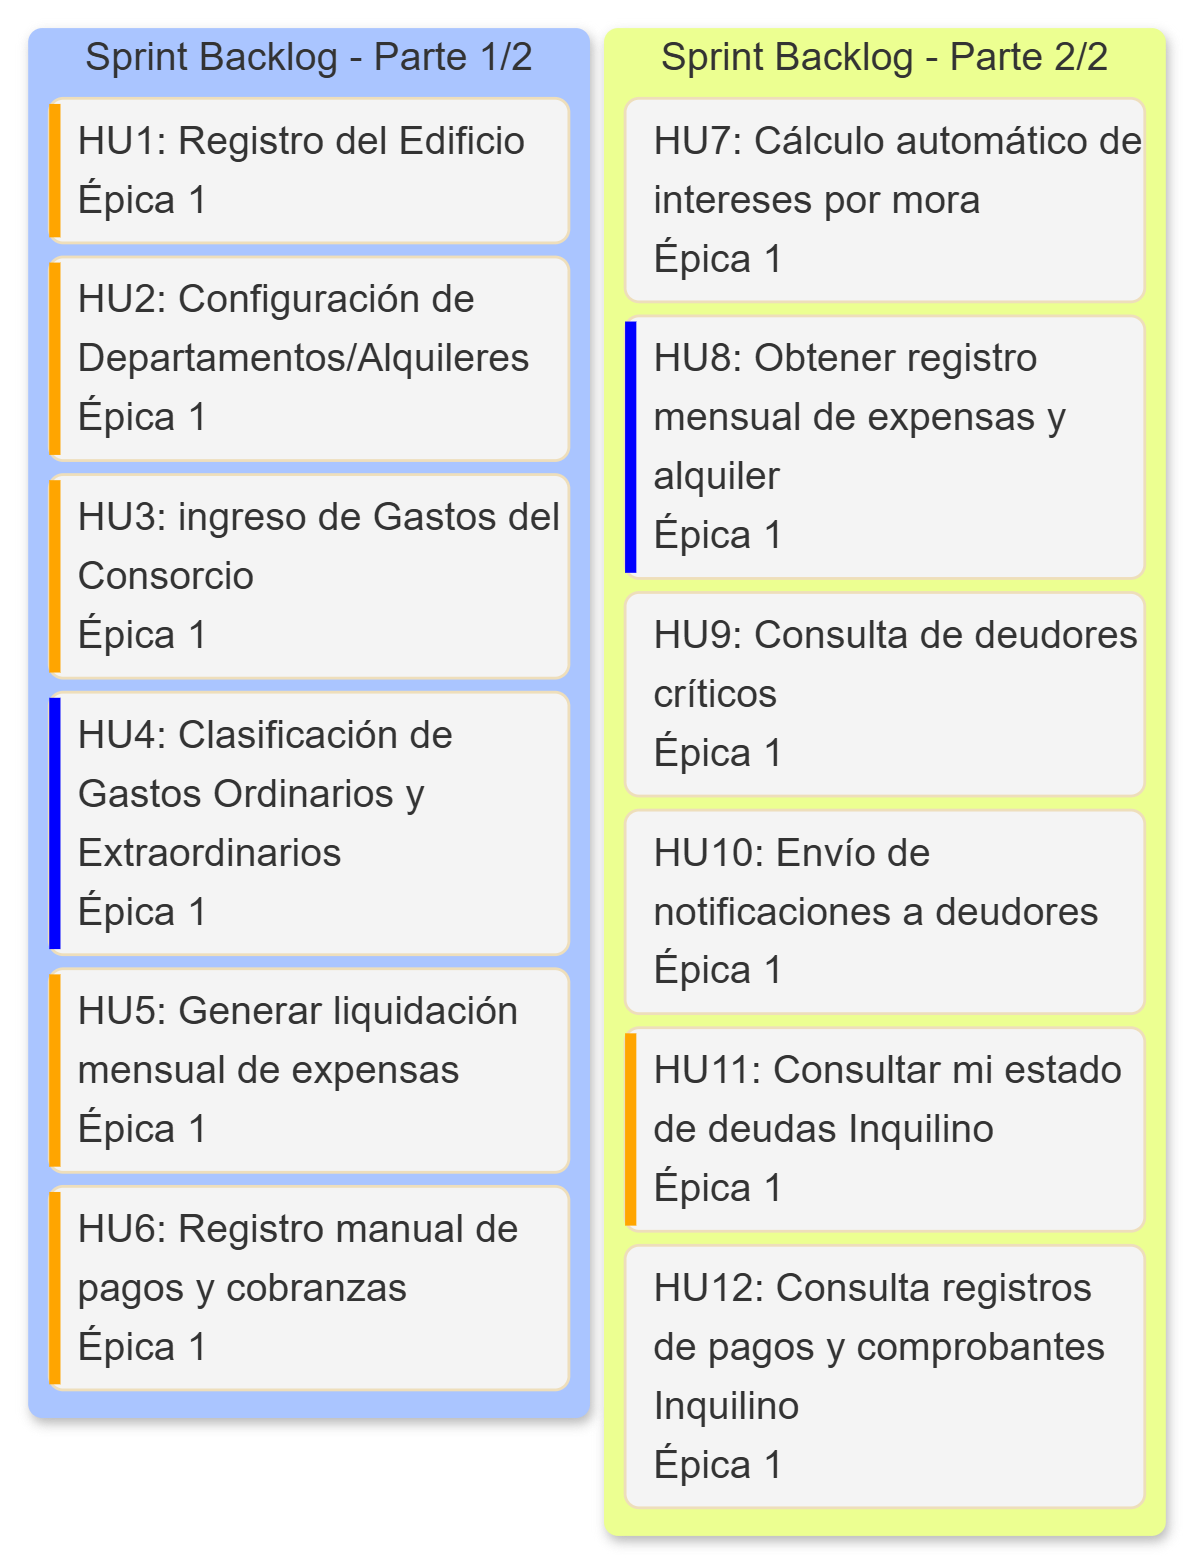
\includegraphics[width=0.7\textwidth]{figures/sprint-backlog.png}
    \caption{Mapeo de Historias de Usuario.}
\end{figure}

\paragraph{Estimación de Historias de Usuario.}
Se aplicó la técnica de \textbf{Estimación por afinidad} (Affinity Estimation), categorizando el esfuerzo y complejidad técnica del Product Backlog en tamaños relativos (Pequeño, Mediano, Grande). Esto permite al equipo alinear expectativas rápidamente, detectando que los módulos contables de prorrateo de expensas e integración de pagos representan las historias de mayor tamaño y riesgo técnico (Grande), mientras que los módulos de comunicación estimaron un esfuerzo menor (Pequeño).


\begin{figure}[H]
    \centering
    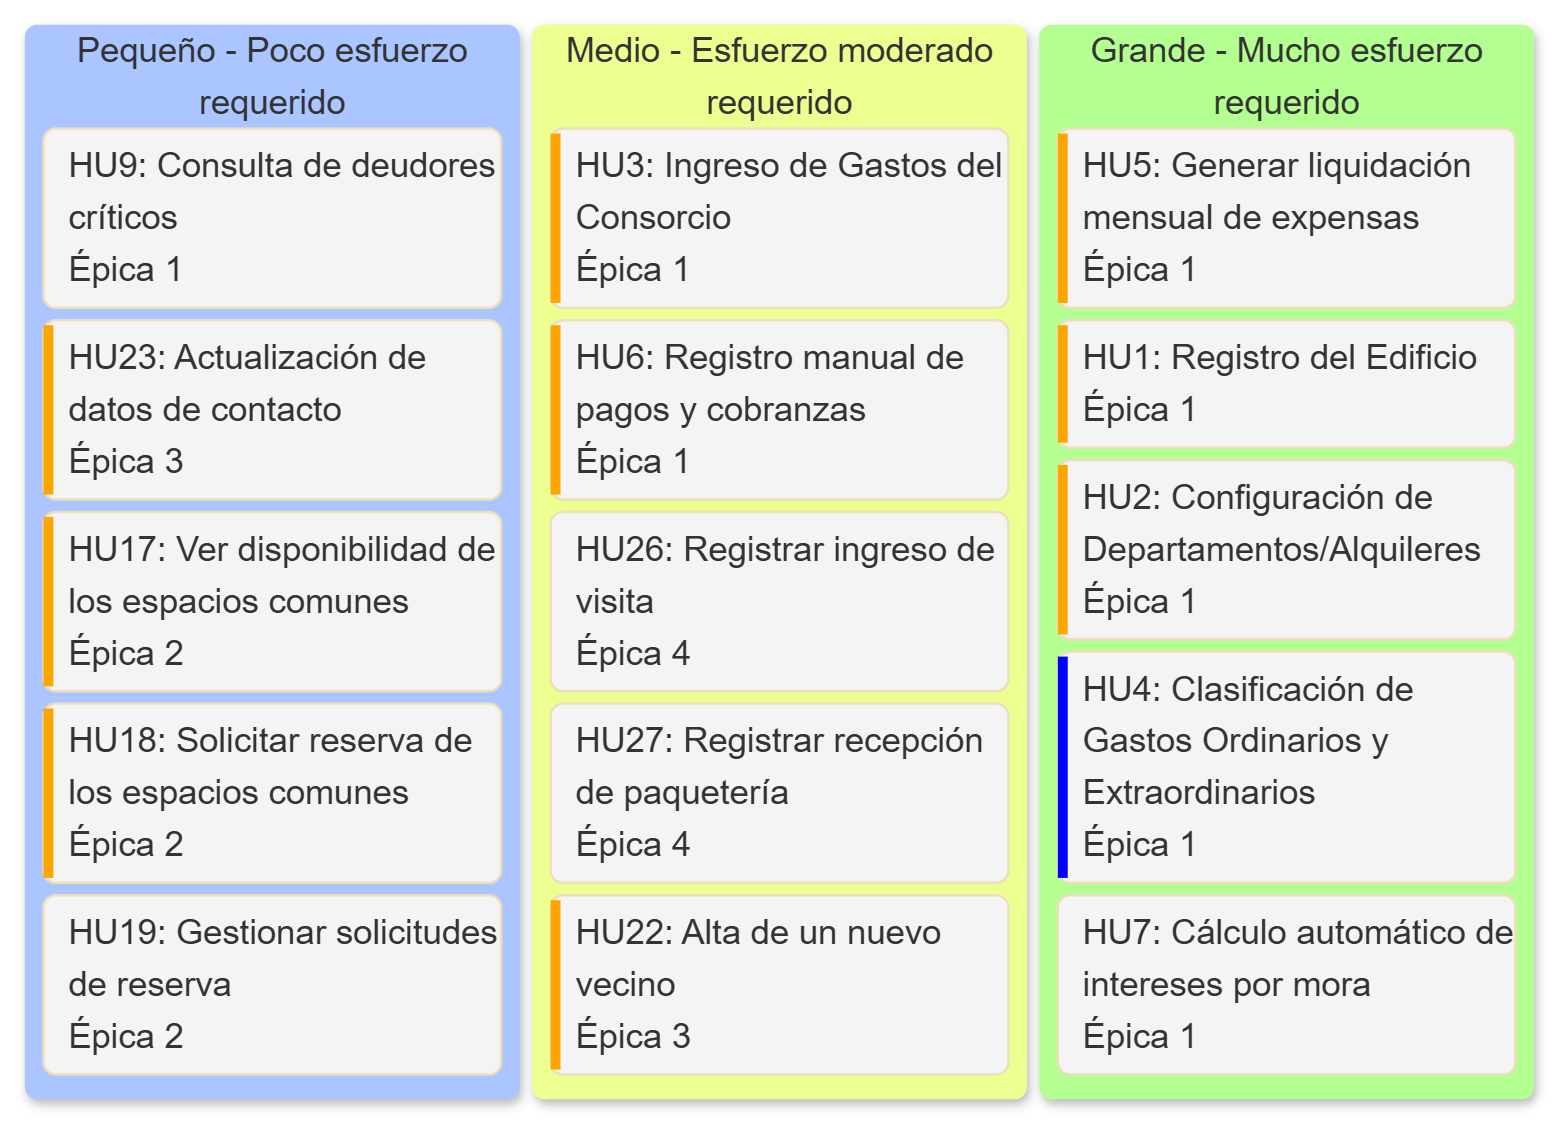
\includegraphics[width=0.8\textwidth]{figures/simulacion-de-estimacion-por-afinidad-en-trello.png}
    \caption{Simulación de Estimación por afinidad en Trello.}
\end{figure}

\paragraph{Compromiso de Historias de Usuario.}
Una vez priorizado el producto backlog y estimado el esfuerzo mediante la técnica de afinidad, el Equipo Scrum llevó a cabo la reunión de planificación del Sprint. El objetivo de la reunión fue definir el \textbf{Sprint Backlog} para el primer ciclo de desarrollo (Sprint 1), el cual cuenta con un Time-boxing de dos semanas.

Durante este proceso, el Equipo de Desarrollo evaluó su capacidad operativa y procedió a mover las historias de usuario de mayor prioridad desde la cima del Product Backlog hacia el Sprint Backlog.

Para el \textbf{Sprint 1 de la Liberación 1}, el equipo se ha comprometido formalmente a implementar las Historias de Usuario HU1 - Registro del Edificio, HU2 - Configuración de Departamentos/Alquileres, HU5 - Generar liquidación mensual de expensas, HU3 - ingreso de Gastos del Consorcio y HU6: Registro manual de pagos y cobranzas. Al tratarse de requerimientos de tamaño ``Grande'' y ``Mediano'' respectivamente, se determinó que estas historias cubren la capacidad de trabajo del equipo para esta primera iteración.

Para el \textbf{Sprint 2 de la Liberación 1}, el equipo se ha comprometido formalmente a implementar las Historias de Usuario, HU11: Consultar mi estado de deudas (Inquilino), HU15: Consultar gastos de expensa mensual (Inquilino) y HU13 - Pagar de deudas Online (Inquilino). Al tratarse de requerimientos de tamaños ``Mediano'' y ``Pequeño'', se determinó que estas historias cubren la capacidad de trabajo del equipo en esta segunda iteración.

Para el \textbf{Sprint 1 de la Liberación 2}, el equipo se ha comprometido formalmente a implementar las Historias de Usuario HU17 - Ver disponibilidad de los espacios comunes, HU18 - Solicitar reserva de los espacios comunes y HU20 - Cancelar reserva del espacio común. Se determinó que estas historias cubren la capacidad de trabajo del equipo para esta primera iteración.

Para el \textbf{Sprint 2 de la Liberación 2}, el equipo se ha comprometido formalmente a implementar Historias de Usuario HU22 - Alta de un nuevo vecino, HU23 - Actualización de datos de contacto y HU24 - Baja o desvinculación de un inquilino. Se determinó que estas historias cubren la capacidad de trabajo del equipo para esta segunda iteración.

Para el \textbf{Sprint 1 de la Liberación 3}, el equipo se ha comprometido formalmente a implementar Historias de Usuario HU26 - Registrar ingreso de visita, HU27 - Registrar recepción de paquetería y HU28 - Confirmar retiro de paquete. Se determinó que estas tareas son las que cubren la capacidad de trabajo del equipo para la primera iteración.

Para el \textbf{Sprint 2 de la Liberación 3}, el equipo se ha comprometido formalmente a implementar Historias de Usuario HU29 - Publicar un comunicado general, HU30 - Consultar documentos del consorcio y HU31 - Enviar consulta directa a la administración. Se determinó que estas tareas son las que cubren la capacidad de trabajo del equipo para la segunda iteración.

\paragraph{Identificación de Tareas.}

\begin{longtable}{|p{4.5cm}|p{10.5cm}|}
    \hline
    \textbf{Historias de Usuario} & \textbf{Tareas técnicas identificadas}
    \\ \hline
    \endhead

        \textbf{HU1 - Registro del Edificio} 
        
        & 

            \begin{enumerate}[leftmargin=*,nosep]
                \item Diseñar tabla \textit{edificios} en la base de datos.
                \item Crear Modelo y Controlador en Laravel.
                \item Desarrollar formulario de Registro (HTML/Blade).
                \item Implementar validaciones de campos (Nombre, CUIT, Dirección).
                \item Realizar pruebas de persistencia de datos.
            \end{enumerate} 
        
    \\ \hline

        \textbf{HU2: Configuración de Departamentos/Alquileres} 
        
        & 

            \begin{enumerate}[leftmargin=*,nosep]
                \item Diseñar tabla unidades \textit{vinculada} a \textit{edificios} en la base de datos.
                \item Crear lógica de asignación de coeficientes (porcentaje de las expensas).
                \item Desarrollar vista de listado de departamentos.
            \end{enumerate} 
        
    \\ \hline

        \textbf{HU3: Ingreso de Gastos del Consorcio.} 
        
        & 

            \begin{enumerate}[leftmargin=*,nosep]
                \item Diseñar tabla \textit{gastos\_consorcio}.
                \item Crear formulario de carga de facturas (Monto, Fecha, Concepto) y sección de carga de archivos.
                \item Implementar lógica de suma automática de gastos del mes.
            \end{enumerate} 
        
    \\ \hline

        \textbf{HU5 - Generar liquidación mensual de expensas} 
        
        & 

            \begin{enumerate}[leftmargin=*,nosep]
                \item Diseñar tabla \textit{liquidaciones} en la base de datos.
                \item \textbf{Crear vista (FrontEnd):} maquetar la pantalla del panel de administración que contenga el botón ``Cerrar mes'' y la ventana emergente de confirmación.
                \item \textbf{Desarrollar lógica de sumatoria (BackEnd):} programar en el controlador la consulta que sume todos los gastos cargados en el mes actual.
                \item \textbf{Desarrollar algoritmo de prorrateo:} Crear la función que tome el total de gastos y lo multiplique por el coeficiente (porcentaje) de cada unidad funcional para sacar el individual.
                \item \textbf{Generar recibos digitales:} maquetar la vista o el PDF del comprobante que verá el inquilino con su monto detallado.
                \item \textbf{Implementar validación de seguridad:} programar un bloqueo para que el administrador no pueda hacer clic en ``Cerrar mes'' dos veces para el mismo período (evitar duplicar deudas).
            \end{enumerate} 
        
    \\ \hline

        \textbf{HU6 - Registro manual de pagos y cobranzas} 
        
        & 

            \begin{enumerate}[leftmargin=*,nosep]
                \item \textbf{Diseñar} tabla \textit{pagos} en la base de datos.
                \item \textbf{Crear formulario de cobro (FrontEnd/Blade):} maquetar la pantalla para el administrador (menú desplegable de departamento y campo de monto).
                \item \textbf{Desarrollar la lógica de guardado (Backend/Controlador):} Escribir la función que guarde los datos del formulario en la tabla \textit{pagos}.
                \item \textbf{Actualizar el pago de la deuda (BackEnd):} programar lógica que busque la liquidación de ese mes y cambie el estado de ``Pendiente'' a ``Pagado''.
                \item \textbf{Generar comprobante Interno:} Maquetar una vista sencilla que muestre un resumen del pago exitoso.
            \end{enumerate} 
        
    \\ \hline

        \textbf{HU11 - Consultar mi estado de deudas (Inquilino)} 
        
        & 

            \begin{enumerate}[leftmargin=*,nosep]
                \item \textbf{Desarrollar consulta a la base de datos (BackEnd/Controlador):} buscar en la tabla de \textit{liquidaciones} el registro actual de la unidad funcional.
                \item \textbf{Crear vista principal (FrontEnd/Blade):} maquetar la pantalla ``Mis deudas'' en el panel del inquilino.
                \item \textbf{Programar lógica condicional en la Vista:} evaluar si el estado de la liquidación es ``Pendiente'' o ``Pagado''.
                \item \textbf{Maquetar escenario ``Con Deuda'' (Frontend):} diseñar la tarjeta de alerta con monto y vencimiento.
                \item \textbf{Maquetar escenario ``Sin Deuda'' (FrontEnd):} diseñar el mensaje de éxito (``Estás al día'').
            \end{enumerate} 
        
    \\ \hline

        \textbf{HU15 - Consultar gastos de expensa mensual (Inquilino)} 
        
        & 

            \begin{enumerate}[leftmargin=*,nosep]
                \item \textbf{Crear botón de acción (FrontEnd):} agregar el enlace ``ver detalle de gastos'' en la liquidación del inquilino.
                \item \textbf{Desarrollar consulta relacional (BackEnd):} buscar en la tabla \textit{gastos\_consorcio} las facturas correspondientes al mes/año.
                \item \textbf{Maquetar vista de detalle (FrontEnd):} diseñar una ventana emergente o tabla desplegable.
                \item \textbf{Formatear la salida de datos:} configurar columnas claras (Fecha, concepto, comprobante, monto) y sumatoria coincidente.
            \end{enumerate} 
        
    \\ \hline

        \textbf{HU13 - Pagar de deudas Online (Inquilino)} 
        
        & 

            \begin{enumerate}[leftmargin=*,nosep]
                \item \textbf{Investigar e integrar API de pagos:} Configurar credenciales (Tokens/Keys) en el archivo `.env`.
                \item \textbf{Crear botón de pago (Frontend/Blade):} Implementar el botón ``Pagar ahora'' capturando el monto adeudado.
                \item \textbf{Desarrollar Controlador de Integración (Backend):} Enviar datos de la deuda a la API y generar el enlace de pago seguro.
                \item \textbf{Implementar \textit{Webhook} para confirmación (Backend):} Programar ruta para recibir notificaciones de la pasarela.
                \item \textbf{Programar lógica de éxito:} Actualizar estado a ``Pagado'' al recibir estado ``Aprobado''.
                \item \textbf{Programar lógica de fallo:} Mantener estado ``Pendiente'' y mostrar error en caso de rechazo.
            \end{enumerate} 
        
    \\ \hline

        \textbf{HU18 - Solicitar reserva de los espacios comunes} 
        
        & 

            \begin{enumerate}[leftmargin=*,nosep]
                \item \textbf{Diseñar tabla en base de datos (reservas):} Crear la migración con campos requeridos.
                \item \textbf{Crear formulario de solicitud (Frontend/Blade):} Maquetar formulario con selector de fecha, invitados y reglamento.
                \item \textbf{Desarrollar lógica de validación (Backend/Controlador):} Validar fecha a futuro, checkbox y límite de invitados.
                \item \textbf{Programar lógica de guardado (Backend):} Persistir la reserva con estado inicial ``Pendiente''.
                \item \textbf{Implementar disparador de notificación (Backend):} Generar alerta interna o enviar correo al Administrador al guardar.
            \end{enumerate} 
        
    \\ \hline

        \textbf{HU20 - Cancelar reserva del espacio común} 
        
        & 

            \begin{enumerate}[leftmargin=*,nosep]
                \item \textbf{Crear interfaz de cancelación (Frontend/Blade):} Agregar botón ``Cancelar Reserva'' en reservas activas.
                \item \textbf{Desarrollar lógica de cálculo de tiempo (Backend/Controlador):} Calcular diferencia en horas respecto a la reserva.
                \item \textbf{Implementar validación condicional (Backend):} Evaluar si la diferencia es mayor a 48 horas.
                \item \textbf{Programar escenario de éxito (Criterio 1):} Actualizar estado a ``Cancelada'' y notificar al administrador.
                \item \textbf{Programar escenario de rechazo (Criterio 2):} Abortar transacción y retornar error en vista.
                \item \textbf{Maquetar alertas de retroalimentación (Frontend):} Diseñar notificaciones visuales para éxito o plazo expirado.
            \end{enumerate} 
        
    \\ \hline

        \textbf{HU17 - Ver disponibilidad de los espacios comunes} 
        
        & 

            \begin{enumerate}[leftmargin=*,nosep]
                \item \textbf{Integrar componente de calendario (Frontend):} Instalar y configurar *FullCalendar.js*.
                \item \textbf{Desarrollar consulta de rango de fechas (Backend):} Buscar reservas del mes/año actual en la base de datos.
                \item \textbf{Mapear estados de disponibilidad (Lógica de Interfaz):} Asignar clases CSS verde (disponible) o rojo (reservado/pendiente).
                \item \textbf{Programar enrutamiento:} Redirigir al clic en verde a ``Nueva Reserva'' con fecha pre-cargada.
                \item \textbf{Bloquear interacción:} Deshabilitar clics en rojo y días pasados.
            \end{enumerate} 
        
    \\ \hline

        \textbf{HU22 - Alta de un nuevo vecino} 
        
        & 

            \begin{enumerate}[leftmargin=*,nosep]
                \item \textbf{Diseñar estructura de usuarios (Base de Datos):} UNIQUE en `dni` y `email` en la tabla `users`.
                \item \textbf{Crear formulario de Alta (Frontend/Blade):} Campos de Nombre, DNI, Email y selector de unidad funcional.
                \item \textbf{Desarrollar lógica de validación (Backend/Controlador):} Validar en servidor que DNI y email sean únicos.
                \item \textbf{Programar generación de credenciales (Backend):} Generar contraseña aleatoria y encriptarla al crear el perfil.
                \item \textbf{Implementar servicio de mensajería (Backend/Mailable):} Enviar correo de bienvenida con credenciales al nuevo inquilino.
            \end{enumerate} 
        
    \\ \hline

        \textbf{HU24 - Baja o desvinculación de un inquilino} 
        
        & 

            \begin{enumerate}[leftmargin=*,nosep]
                \item \textbf{Maquetar interfaz de desvinculación (Frontend/Blade):} Botón ``Dar de baja'' y modal de confirmación.
                \item \textbf{Desarrollar lógica de Borrado Lógico (Backend):} Cambiar estado a ``Inactivo'' preservando historial.
                \item \textbf{Actualizar estado de la Unidad Funcional (Backend):} Desvincular usuario del departamento y marcarlo ``Desocupada''.
                \item \textbf{Implementar revocación de sesión activa (Seguridad):} Middleware para expulsar al usuario si está logueado.
            \end{enumerate} 
        
    \\ \hline

        \textbf{HU23 - Actualización de datos de contacto} 
        
        & 

            \begin{enumerate}[leftmargin=*,nosep]
                \item \textbf{Crear vista ``Mi Perfil'' (Frontend/Blade):} Formulario pre-cargado con información actual.
                \item \textbf{Desarrollar enrutamiento protegido (Backend):} Proteger la ruta para usuarios logueados.
                \item \textbf{Programar validación y sanitización (Backend/Controlador):} Validar formato de email y caracteres del teléfono.
                \item \textbf{Ejecutar actualización segura (Backend):} Actualizar únicamente teléfono y email del usuario logueado.
                \item \textbf{Implementar retroalimentación visual (Frontend):} Retornar a la vista con mensaje de éxito (Toast/Alert).
            \end{enumerate} 
        
    \\ \hline

        \textbf{HU26 - Registrar ingreso de visita} 
        
        & 

            \begin{enumerate}[leftmargin=*,nosep]
                \item \textbf{Diseñar tabla de auditoría (visitas):} Crear migración con campos necesarios.
                \item \textbf{Crear vista para el rol Guardia (Frontend/Blade):} Maquetar panel rápido ``Libro de Visitas''.
                \item \textbf{Desarrollar lógica de persistencia (Backend/Controlador):} Registrar datos del formulario de visitas.
                \item \textbf{Implementar sellado de tiempo automático:} Capturar hora de ingreso del servidor.
                \item \textbf{Configurar estado inicial:} Guardar con estado por defecto ``En el edificio''.
                \item \textbf{Maquetar tabla de visitas activas (Frontend):} Lista de visitas en tiempo real.
            \end{enumerate} 
        
    \\ \hline

        \textbf{HU27 - Registrar recepción de paquetería} 
        
        & 

            \begin{enumerate}[leftmargin=*,nosep]
                \item \textbf{Diseñar tabla de inventario (paquetes):} Crear migración con campos y estado ``En guardia''.
                \item \textbf{Crear formulario de recepción (Frontend/Blade):} Campos de remitente y selector de departamento.
                \item \textbf{Desarrollar Controlador de registro (Backend):} Validar e ingresar paquete asociado a la unidad.
                \item \textbf{Desarrollar lógica de notificación asíncrona (Backend):} Evento y Listener para notificar al inquilino por correo/alerta.
            \end{enumerate} 
        
    \\ \hline

        \textbf{HU28 - Confirmar retiro de paquete} 
        
        & 

            \begin{enumerate}[leftmargin=*,nosep]
                \item \textbf{Modificar vista de inventario (Frontend/Blade):} Agregar botón ``Marcar como Entregado''.
                \item \textbf{Desarrollar ruta y Controlador (Backend):} Crear método que reciba el ID del paquete.
                \item \textbf{Implementar lógica de actualización y auditoría (Backend):} Cambiar estado a ``Entregado'' y registrar hora.
                \item \textbf{Ajustar consulta de filtrado (Backend/Controlador):} Filtrar paquetes entregados de la lista de pendientes de guardia.
            \end{enumerate} 
        
    \\ \hline

        \textbf{HU29 - Publicar un comunicado general} 
        
        & 

            \begin{enumerate}[leftmargin=*,nosep]
                \item \textbf{Diseñar tabla de anuncios (comunicados):} Crear migración con campos y autor.
                \item \textbf{Crear formulario de publicación (Frontend/Blade - Admin):} Formulario para redactar avisos.
                \item \textbf{Desarrollar lógica de persistencia (Backend/Controlador):} Validar y guardar comunicado.
                \item \textbf{Implementar Colas de Trabajo (Backend):} Job para enviar correos masivos de forma asíncrona.
                \item \textbf{Modificar el Dashboard del inquilino (Frontend/Blade):} Renderizar últimos comunicados en la página de inicio.
            \end{enumerate} 
        
    \\ \hline

        \textbf{HU31: Enviar consulta directa a la administración} 
        
        & 

            \begin{enumerate}[leftmargin=*,nosep]
                \item \textbf{Diseñar tabla de mensajería (tickets o consultas):} Migración con campos e inquilino\_id.
                \item \textbf{Crear formulario de contacto (Frontend/Blade - Inquilino):} Formulario para redactar consultas.
                \item \textbf{Desarrollar lógica de persistencia (Backend/Controlador):} Guardar consulta asociada al usuario logueado.
                \item \textbf{Maquetar bandeja de entrada (Frontend/Blade - Admin):} Bandeja ordenada por fecha de creación.
                \item \textbf{Desarrollar consulta de tickets (Backend/Controlador):} Query para listar y filtrar por estado (Pendiente/Resuelto).
            \end{enumerate} 
        
    \\ \hline

        \textbf{HU30 - Consultar documentos del consorcio} 
        
        & 

            \begin{enumerate}[leftmargin=*,nosep]
                \item \textbf{Diseñar tabla de metadatos (documentos):} Crear migración con título, path y fecha.
                \item \textbf{Crear vista de repositorio (Frontend/Blade):} Grilla con íconos de los documentos del consorcio.
                \item \textbf{Desarrollar consulta de listado (Backend/Controlador):} Recuperar y enviar documentos públicos a la vista.
                \item \textbf{Implementar lógica de entrega de archivos (Backend):} Ruta de descarga segura utilizando la clase Storage.
                \item \textbf{Configurar cabeceras de respuesta HTTP:} response()-\>file() para visualización inline en el navegador.
            \end{enumerate} 
        
    \\ \hline

    \caption{Tabla de identificación de Tareas}
\end{longtable}

\paragraph{Estimación de Tareas}

\begin{longtable}{|p{10.5cm}|p{2.5cm}|c|}
    \hline
            \textbf{Historia de Usuario} 
        & 
            \textbf{Estimación de Tareas} 
        & 
            \textbf{Estimación total} 
    \\ \hline
    \endhead

            \textbf{HU1 - Registro del Edificio} 
        
        & 

            \begin{enumerate}[leftmargin=*,nosep]
                \item 2 h
                \item 1 h
                \item 2 h
                \item 3 h
                \item 2 h
            \end{enumerate} 
        
        &
        
            10 h 
        
    \\ \hline
        
            \textbf{HU2 - Configuración de Departamentos/Alquileres} 
        
        &

            \begin{enumerate}[leftmargin=*,nosep]
                \item 2 h
                \item 2 h
                \item 2 h
            \end{enumerate} 
        
        &
            8 h
    
    \\ \hline
        
            \textbf{HU3 - Ingreso de Gastos del Consorcio.} 
        
        &

            \begin{enumerate}[leftmargin=*,nosep]
                \item 2 h
                \item 1 h
                \item 2 h
            \end{enumerate} 
        
        &
            5 h
    
    \\ \hline
        
            \textbf{HU5 - Generar liquidación mensual de expensas} 
        
        &

            \begin{enumerate}[leftmargin=*,nosep]
                \item 2 h
                \item 2 h
                \item 2 h
                \item 3 h
                \item 1 h
                \item 2 h
            \end{enumerate} 
        
        &
         12 h
    \\ \hline
        
            \textbf{HU6 - Registro manual de pagos y cobranzas} 
        
        &

            \begin{enumerate}[leftmargin=*,nosep]
                \item 2 h
                \item 2 h
                \item 3 h
                \item 1 h
                \item 2 h
            \end{enumerate} 
        
        &
         10 h
    \\ \hline
        
            \textbf{HU11 - Consultar mi estado de deudas (Inquilino)} 
        
        &

            \begin{enumerate}[leftmargin=*,nosep]
                \item 2 h
                \item 2 h
                \item 1 h
                \item 3 h
                \item 2 h
            \end{enumerate} 
        
        &
            10 h
    
    \\ \hline
        
            \textbf{HU15 - Consultar gastos de expensa mensual (Inquilino)} 
        
        &

            \begin{enumerate}[leftmargin=*,nosep]
                \item 1 h
                \item 2 h
                \item 3 h
                \item 3 h
            \end{enumerate} 
        
        &
            9 h
    
    \\ \hline
        
            \textbf{HU13 - Pagar de deudas Online (Inquilino)} 
        
        &

            \begin{enumerate}[leftmargin=*,nosep]
                \item 3 h
                \item 2 h
                \item 3 h
                \item 2 h
                \item 2 h
                \item 3 h
            \end{enumerate} 
        
        &
            15 h
    
    \\ \hline
        
            \textbf{HU18 - Solicitar reserva de los espacios comunes} 
        
        &

            \begin{enumerate}[leftmargin=*,nosep]
                \item 2 h
                \item 3 h
                \item 4 h
                \item 3 h
                \item 3 h
            \end{enumerate} 
        
        &
            15 h
    
    \\ \hline
        
            \textbf{HU20 - Cancelar reserva del espacio común} 
        
        &

            \begin{enumerate}[leftmargin=*,nosep]
                \item 1 h
                \item 3 h
                \item 4 h
                \item 3 h
                \item 2 h
                \item 2 h
            \end{enumerate} 
        
        &
            15 h
    
    \\ \hline
        
            \textbf{HU17 - Ver disponibilidad de los espacios comunes} 
        
        &

            \begin{enumerate}[leftmargin=*,nosep]
                \item 2 h
                \item 3 h
                \item 3 h
                \item 4 h
                \item 3 h
            \end{enumerate} 
        
        &
            15 h
    
    \\ \hline
        
            \textbf{HU22 - Alta de un nuevo vecino} 
        
        &

            \begin{enumerate}[leftmargin=*,nosep]
                \item 2 h
                \item 2 h
                \item 3 h
                \item 4 h
                \item 5 h
            \end{enumerate} 
        
        &
            16 h
    
    \\ \hline
        
            \textbf{HU24 - Baja o desvinculación de un inquilino} 
        
        &

            \begin{enumerate}[leftmargin=*,nosep]
                \item 2 h
                \item 3 h
                \item 3 h
                \item 2 h
            \end{enumerate} 
        
        &
            10 h
    
    \\ \hline
        
            \textbf{HU23 - Actualización de datos de contacto} 
        
        &

            \begin{enumerate}[leftmargin=*,nosep]
                \item 2 h
                \item 2 h
                \item 3 h
                \item 3 h
                \item 3 h
            \end{enumerate} 
        
        &
            13 h
    
    \\ \hline
        
            \textbf{HU26 - Registrar ingreso de visita} 
        
        &

            \begin{enumerate}[leftmargin=*,nosep]
                \item 2 h
                \item 3 h
                \item 3 h
                \item 4 h
                \item 5 h
                \item 3 h
            \end{enumerate} 
        
        &
            20 h
    
    \\ \hline
        
            \textbf{HU27 - Registrar recepción de paquetería} 
        
        &

            \begin{enumerate}[leftmargin=*,nosep]
                \item 2 h
                \item 3 h
                \item 4 h
                \item 3 h
            \end{enumerate} 
        
        &
            12 h
    
    \\ \hline
        
            \textbf{HU28 - Confirmar retiro de paquete} 
        
        &

            \begin{enumerate}[leftmargin=*,nosep]
                \item 2 h
                \item 3 h
                \item 5 h
                \item 4 h
            \end{enumerate} 
        
        &
            14 h
    
    \\ \hline
        
            \textbf{HU29 - Publicar un comunicado general} 
        
        &

            \begin{enumerate}[leftmargin=*,nosep]
                \item 2 h
                \item 3 h
                \item 4 h
                \item 5 h
                \item 4 h
            \end{enumerate} 
        
        &
            18 h
    
    \\ \hline
        
            \textbf{HU31 - Enviar consulta directa a la administración} 
        
        &

            \begin{enumerate}[leftmargin=*,nosep]
                \item 3 h
                \item 3 h
                \item 3 h
                \item 2 h
                \item 2 h
            \end{enumerate} 
        
        &
            13 h
    
    \\ \hline
        
            \textbf{HU30 - Consultar documentos del consorcio} 
        
        &

            \begin{enumerate}[leftmargin=*,nosep]
                \item 2 h
                \item 3 h
                \item 4 h
                \item 3 h
                \item 2 h
            \end{enumerate} 
        
        &
            14 h
    
    \\ \hline
        
        &

        \begin{enumerate}[leftmargin=*,nosep]
          \item 2 h
          \item 3 h
          \item 4 h
          \item 3 h
          \item 2 h
        \end{enumerate} 
        
        &
         14 h \\ \hline
        
    \caption{Tabla de estimación de tareas.}
\end{longtable}

\paragraph{Actualizar el backlog del sprint}
Dado que la Liberación 1 está planificada para durar un mes en total, se dividió el trabajo en 2 Sprints de dos semanas de duración cada uno. Para el \textbf{Sprint 1}, el Backlog del Sprint se actualizó trasladando las tareas técnicas (previamente identificadas en Trello) correspondientes a las historias fundamentales (Registro de Edificio, Configuración de Unidades, Ingreso de Gastos y Liquidación Mensual). El resto de las historias de la Liberación 1 (como Consultar deudas y Pagar online) quedaron reservadas para la planificación del Sprint 2.

\subsubsection{2.1.3 - Fase - Implementación}

\paragraph{Crear entregables.}
Los desarrolladores proceden a la codificación en el framework Laravel, creando las migraciones de bases de datos, maquetando las vistas (Frontend) y programando los Controladores. A medida que las tareas avanzan, las tarjetas en el tablero Trello se mueven de la columna ``Por hacer'' a ``En progreso'' y finalmente a ``Terminada''. 

\paragraph{Realizar el Daily Standup.}
El equipo de desarrollo realiza una reunión diaria de máximo 15 minutos donde cada integrante responde tres preguntas clave: ¿Qué hice ayer para ayudar a terminar el Sprint?, ¿Qué haré hoy?, y ¿Existe algún impedimento que me bloquee? 

\paragraph{Refinar el backlog priorizado del producto.}
El Product Owner revisa las historias de usuario de futuras épicas (como el módulo del Personal de Seguridad) para asegurar que estén claras y listas para cuando inicie la planificación de las siguientes iteraciones.

\subsubsection{2.1.4 - Fase - Revisión y Retrospectiva}

\paragraph{Demostrar y validar el sprint.}
Se realiza una demostración del software funcional. Por ejemplo, el equipo muestra cómo el sistema logra tomar los gastos cargados y generar exitosamente la liquidación mensual prorrateada. Si cumple con los Criterios de Aceptación, la historia se marca como ``Hecha''. 

\paragraph{Retrospectiva del sprint.}
El equipo evalúa sus procesos internos. Se identifican aspectos positivos (ej. ``usar migraciones de Laravel agilizó el trabajo'') y áreas de mejora (ej. ``subestimamos el tiempo que tomaba maquetar las vistas'') para aplicar correcciones de cara al Sprint 2.

\subsubsection{2.1.5 - Fase - Liberación}

\paragraph{Enviar Entregables.}
El código fuente se despliega en un servidor de producción. A partir de este momento, la administración del consorcio ya cuenta con un incremento de producto funcional que pueden utilizar en su día a día para gestionar los edificios y las liquidaciones, mientras el equipo de desarrollo comienza a trabajar en la Liberación 2 (Módulo de reservas). 

\paragraph{Retrospectiva de la liberación.}
Tras completar la totalidad de las iteraciones planeadas para el cuatrimestre, se realiza una reunión global final. Se documenta la experiencia general, evaluando si el sistema cumplió con la visión original y analizando el impacto positivo de haber utilizado un marco de trabajo ágil e iterativo frente a las metodologías tradicionales.

